% Propósito: distinguir nivel del enmascarador, umbral enmascarado y elevación
% del umbral, y relacionar la selectividad de un filtro auditivo con su ERB.
% Origen: M(f_s)=L_umbral,e(f_s)-L_umbral,q(f_s), ecuación
% \eqref{eq:u7-elevacion-umbral}, y definición de ERB de la sección
% \ref{sec:u7-filtros-auditivos}. Curvas cualitativas; no son mediciones.
% Descripción accesible: el panel izquierdo muestra un umbral en quietud, un
% enmascarador y un umbral elevado; una flecha vertical marca M en la frecuencia
% de la señal objetivo. El panel derecho muestra la respuesta normalizada de un
% filtro y un rectángulo con la misma altura máxima y la misma área; su ancho es
% la ERB.
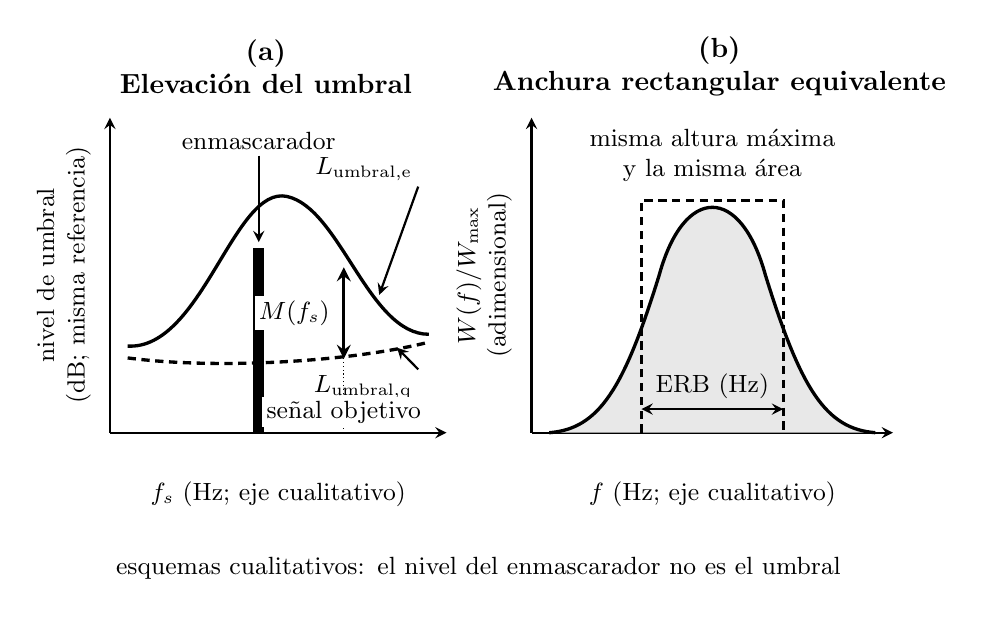
\begin{tikzpicture}[font=\small,>=stealth,x=0.90cm,y=1cm]
    \node[font=\bfseries,align=center] at (3.00,5.75)
        {(a)\\Elevación del umbral};
    \draw[->,thick] (0.80,1.10) -- (5.55,1.10)
        node[pos=0.50,below=14pt]
        {\(f_s\) (Hz; eje cualitativo)};
    \draw[->,thick] (0.80,1.10) -- (0.80,5.10);
    \node[rotate=90,align=center] at (0.15,3.10)
        {nivel de umbral\\(dB; misma referencia)};

    \draw[very thick,densely dashed]
        (1.05,2.05) .. controls (2.30,1.90) and (4.20,2.00) .. (5.30,2.25);
    \draw[very thick]
        (1.05,2.20) .. controls (2.10,2.15) and (2.55,4.25) ..
        (3.30,4.10) .. controls (4.05,3.95) and (4.45,2.35) ..
        (5.30,2.35);
    \draw[line width=4pt] (2.90,1.10) -- (2.90,3.45);
    \node[anchor=south,fill=white,inner sep=2pt]
        (masker-label) at (2.90,4.62) {enmascarador};
    \draw[->,thick] (masker-label.south) -- (2.90,3.52);

    \node[anchor=east,fill=white,inner sep=2pt]
        (masked-threshold-label) at (5.15,4.45)
        {\(L_{\mathrm{umbral,e}}\)};
    \draw[->,thick]
        (masked-threshold-label.south east) -- (4.60,2.85);
    \node[anchor=east,fill=white,inner sep=2pt]
        (quiet-threshold-label) at (5.15,1.68)
        {\(L_{\mathrm{umbral,q}}\)};
    \draw[->,thick]
        (quiet-threshold-label.north east) -- (4.85,2.18);

    \draw[densely dotted] (4.10,1.10) -- (4.10,3.20);
    \draw[<->,very thick] (4.10,2.04) -- (4.10,3.20)
        node[midway,left=3pt,fill=white,inner sep=1.5pt] {\(M(f_s)\)};
    \node[anchor=south,fill=white,inner sep=1.5pt]
        at (4.10,1.16) {señal objetivo};

    \node[font=\bfseries,align=center] at (9.40,5.75)
        {(b)\\Anchura rectangular equivalente};
    \draw[->,thick] (6.75,1.10) -- (11.85,1.10)
        node[pos=0.50,below=14pt]
        {\(f\) (Hz; eje cualitativo)};
    \draw[->,thick] (6.75,1.10) -- (6.75,5.10);
    \node[rotate=90,align=center] at (6.08,3.10)
        {\(W(f)/W_{\max}\)\\(adimensional)};

    \path[fill=black!9]
        (7.00,1.10)
        .. controls (7.70,1.15) and (8.05,1.65) .. (8.55,3.10)
        .. controls (8.90,4.25) and (9.70,4.25) .. (10.05,3.10)
        .. controls (10.55,1.65) and (10.90,1.15) .. (11.60,1.10)
        -- cycle;
    \draw[very thick]
        (7.00,1.10)
        .. controls (7.70,1.15) and (8.05,1.65) .. (8.55,3.10)
        .. controls (8.90,4.25) and (9.70,4.25) .. (10.05,3.10)
        .. controls (10.55,1.65) and (10.90,1.15) .. (11.60,1.10);

    \draw[very thick,densely dashed]
        (8.30,1.10) -- (8.30,4.05) -- (10.30,4.05) -- (10.30,1.10);
    \draw[<->,thick] (8.30,1.40) -- (10.30,1.40)
        node[midway,above] {\(\mathrm{ERB}\) (Hz)};
    \node[align=center] at (9.30,4.62)
        {misma altura máxima\\y la misma área};

    \node[align=center,text width=10.20cm] at (6.00,-0.62)
        {esquemas cualitativos: el nivel del enmascarador no es el umbral};
\end{tikzpicture}
